\documentclass[12pt]{article} 
\usepackage{amsmath} 
\usepackage[dvips]{graphicx}
\usepackage{multirow} 
\usepackage{geometry} 
\usepackage{pdflscape}
\usepackage[labelfont=bf]{caption} 
\usepackage{setspace}
\usepackage[running]{lineno} 
% \usepackage[numbers,sort]{natbib}
\usepackage[round]{natbib} 
\usepackage{array}
\usepackage[table]{xcolor}
\usepackage{xr}

\newcommand{\methods}{\textit{Materials \& Methods}}
\newcommand{\SI}{\textit{Appendix}~}

\topmargin -1.5cm % 0.0cm 
\oddsidemargin 0.0cm % 0.2cm 
\textwidth 6.5in
\textheight 9.0in % 21cm
\footskip 1.0cm % 1.0cm

\usepackage{authblk}

\title{Does motif participation provide unique information about species risk of extinction?}

\author{Anna \r{A}kesson$^{1\dagger}$, Alyssa R. Cirtwill$^{3}$, Kate Wootton$^{2}$, Gyuri Barab\'{a}s$^{1}$, Anna Ekl\"{o}f$^{1}$} 
\date{\small$^1$Department of Theoretical Biology, Chemistry, and Physics\\ 
Link\"{o}ping University\\
Link\"{o}ping, Sweden\\
\medskip
\small$^2$ Swedish Agricultural University\\
Uppsala, Sweden\\
\medskip
\small$^3$Department of Agricultural Sciences\\
University of Helsinki\\
Helsinki, Finland\\
\medskip
$^\dagger$ Corresponding author:\\
}


\begin{document} 
\maketitle 
\raggedright

\setlength{\parindent}{15pt} 
\begin{spacing}{2.0}

% Maybe Proc B - approached Alyssa re: other motifs paper, flexible length limit (but pay extra over X pages).

\section*{Abstract}
    Bottom-up effects of disturbance to basal resources can strongly affect the persistence of consumers.
    However, predicting which species will be most affected by increasing disturbance is not straightforward.
    In-degree and trophic level are known to affect a consumer's vulnerability to bottom-up disturbance, but these are relatively coarse measures of a species' place in a food web.
    Here we explore how roles based on participation in three-species motifs are related to persistence, and how these motif-based roles relate to simpler measures.
    We show that a consumer species' frequency of participation in different motifs is related to its probability of persistence. Similarly, the overall motif profile of a network was related to the average persistence of consumer species.
    Notably, we found that networks containing a higher proportion of the `omnivory' motif tend to have lower mean persistence following disturbance to basal species, while more frequent participation in the omnivory motif was associated with higher probability of persistence.
    Additionally, we find that relationships between motif participation and persistence can synthesize the information provided by in-degree and trophic level.
    Motif participation therefore provides a relatively rich description of a species' structural role in its community and captures important trends in vulnerability to extinction.

    

    Anna AA: The whole article is now approximately 4400 words (not counting fig texts); intro 850, methods 1600, results 620, discussion 1300. See discussion on section statistical analysis in the methods, I think we can make it shorter
    - glossary
    - refs
    - ending


    - Fig. 4 not much in discussion, could be a candidate for the SI? Or add more discussion about apparent competition, etc. in discussion sections per motif

\clearpage
\section*{Introduction}

    %\subsection*{1 Why are bottom-up effects important for understanding stability?}
     The plant community is the foundation upon which the myriad species in terrestrial food webs depend for their survival. Disturbances in the plant community have been shown to affect important ecosystem properties such as primary \citep{Hector1999} and secondary production \citep{borer2012plant}, soil respiration and carbon cycling \citep{chen2019plant} and consumer diversity \citep{scherber2010bottom, Baiser2016}. The stability of the plant community is crucial for sustaining a healthy energy flow in the ecosystem as a whole \citep{Rosenblatt2016} and the structure of the plant community affects stability across all levels of ecosystem organization \citep{proulx2010diversity,scherber2010bottom}. Loss of diversity at the basal level typically causes declines in both abundance and richness of all types of consumers: herbivores, predators,  parasitoids, etc. \citep{scherber2010bottom}.
    
     %\subsection*{2 Bayesian networks are a fantastic way to model bottom-up effects}
    How population decline or extinction of one species leads to loss of other species via direct and indirect effects (i.e., secondary extinctions) is a vibrant area of research \citep{curtsdotter2011robustness, dunne2009cascading, Eklof2006}. Traditionally, there are two main approaches for studying secondary extinctions. First, there are topological models, based only on food web structure \citep{dunne2009cascading}. Here,  extinctions only affect other species in the network once a consumer has lost all of its prey and therefore must go extinct. The second approach uses dynamical models which explicitly simulate population dynamics using a system of differential equations \citep{binzer2011susceptibility}. Dynamical models take changes in prey or predator densities into account when calculating the densities of other species in the network. 
    This additional detail means that realistic processes such as indirect interactions can be included, but also means that dynamical models are more parameter intensive, and simulations are more time-consuming, than topological models. 
    
    
    A middle‐ground approach for simulating secondary extinctions is to use  Bayesian networks \citep{Eklof2013}. 
    In this framework, a consumer's probability of extinction depends on the fraction of resources lost and on a baseline probability of extinction which captures causes unrelated to the network structure (e.g., disease, stochastic extinction of small populations).
    Modelling Bayesian networks is fast and computationally efficient, allowing analysis of networks with high species richness \citep{Haussler2020}. 
    As consumers do not affect the extinction probabilities of their resources, Bayesian networks can only capture bottom-up effects of disturbances within networks. 
    However, Bayesian networks do capture the majority of secondary extinctions captured by dynamical models \citep{Eklof2013}.
    This emphasizes the importance of bottom-up effects in food webs and makes Bayesian networks the ideal framework to use when studying them.  

    %\subsection*{3 Global scale network properties are known to affect stability}
    Using Bayesian networks, researchers can explore how the structures of realistically-large networks shape their responses to disturbance.
    The global (whole-network) structural properties of ecological networks have implications for their functioning \citep{Petchey2002}, stability \citep{Allesina2012} and robustness to disturbances \citep{Dunne2002, Eklof2006}. 
    For example, more highly-connected networks are more resistant to secondary extinctions \citep{Dunne2002, Eklof2006} and a modular organization, where some groups of species are tightly interconnected with limited connections between groups, can limit the propagation of disturbances \citep{Krause2003, Teng2004}.
    
    %\subsection*{4 meso-scale nw propoerties also affect stability}
    Structural properties on the local (single-species) scale are also known to affect response to disturbance. 
    Species with high trophic levels (long paths to basal resources), low in-degree (few prey), and low abundances are generally at higher risks of secondary extinction \citep{binzer2011susceptibility}. 
    However, in-degree and trophic level are both relatively coarse descriptions of a species' role within its food-web~\citep{Cirtwill2018FoodWebs}. 
    For example, a specialist may not necessarily have a high risk of extinction if it consumes a basal resource which is unlikely to be affected by disturbance. 
    On the other hand, a consumer with low trophic level may be at high risk of extinction if it consumes prey which are themselves very likely to be affected by disturbance. 
    
    %\subsection*{5 Motif participation may similarly affect species' particular extinction risk}
    One way to incorporate more nuance into descriptions of how species fit into their communities is to define species' roles based on their participation in different motifs -- unique combinations of small numbers of interacting species~\citep{Stouffer2007,Stouffer2012}. Importantly, these `motif participation roles' capture information about species' direct and indirect interactions, incorporating larger-scale network structure into species-level descriptions~\citep{Cirtwill2015JAE}. 
    This means that two species with the same in-degrees and trophic levels can still participate in different sets of motifs if, for example, one interacts with specialists and the other interacts with generalists~\citep{Cirtwill2018FoodWebs}. 
    This extra detail  may be useful when predicting  extinction risk since, at the network level, the frequencies of different motifs are associated with community stability \citep{prill2005dynamic, bascompte2005simple} and with changes to the composition of plant communities~\cite{giling2019plant}. 
    We therefore expect that the motif structure of a network and species' participation in that structure should be related to risks due to disturbance to basal resources. 
    
           %\subsection*{Here we test...}
    Specifically, we are interested in whether a consumer's extinction risk depends on 1) the motif profile of the full food web and 2) the motifs in which a focal species participates. 
    In addition, we want to understand how the information provided by motifs is related to classical global and local food web properties in order to better synthesize information provided by different scales of network structure.
    Of the 13 three-species motifs that can occur in empirical food webs, there are four motifs that are over-represented in empirical networks and are thought to contribute to stability \citep{Stouffer2007, Borrelli2015a, giling2019plant}. These four motifs, the three-species chain, omnivory, apparent competition, and direct competition, are also the only ones which can occur in the acyclic networks required for Bayesian network simulations~\citep{Eklof2013}. 
    Therefore, we focus on these four particularly important motifs.  
    

    	
\section*{Methods}

	\subsection*{Initial network construction}

		We generated a realistic set of simulated networks based on the niche model~\citep{Williams2000,Stouffer2007} using the function "nichemodel" within the Julia~\citep{Bezanson2017julia} package \emph{BioEnergeticFoodWebs}~\citep{bioenergfw}. 
		To capture a range of plausible network architectures, we simulated networks with sizes ranging from 50 to 100 species (in steps of 10) and connectances ranging from 0.02 to 0.18 (in steps of 0.04). 
		For full details, see~\citet{Cirtwill2021_inprep}.
        We then filtered these simulated networks and removed any network containing disconnected components
        % (species or groups of species not connected to the rest of the network) 
        or any network where any species had a shortest trophic level \textgreater6 as such high trophic levels are very uncommon in empirical food webs ~\citep{Riede2011}.
		New networks were simulated to replace any removed networks, and this process was repeated until we obtained 100 suitable networks in each combination of size and connectance.
		All networks were rendered acyclic following~\citet{Allesina2009} and topologically sorted from lowest to highest trophic level (Appendix\emph{S1}).
		These processing steps allow the strictly bottom-up calculation of probability of persistence used in the Bayesian network framework.
		
% 		A Bayesian food web depicts probabilistic relationships among a set of species where each species' probability of persistence depends upon the probabilities of its resource species persisting~\citep{Jensen_Nielsen,Eklof2013}. 
% 		All persistence calculations therefore begin  by determining the status of the primary producers (who do not depend on other species).
% 		Calculations continue in a strictly bottom-up manner with primary consumers (who depend only on primary producers), and so on up the network.
		
% 		While niche-model food webs can contain cycles (e.g., species A eats B, B eats C, and C eats A), such cycles make it impossible to calculate persistence in the Bayesian network framework~\citep{Tarjan1972}. 
% 		We therefore removed any cycles within each network by removing the link in each cycle which contributed least to the robustness of the food web, following~\citet{Allesina2009}.
% 		%This is achieved by first finding the set of resources for each consumer and then removing the consumer-resource connections which have the lowest eigenvalue centrality~\citep{Allesina2009}.
% 		%These links have the least effect on the overall stability of the network; removing them creates an acyclic network with very similar properties to the original network.
% 		Next, we ordered the species from lowest to highest trophic level using a topological sorting routine following \citep{Tarjan1972, Allesinaetal2005}, ensuring that probability calculations follow a strict bottom-up order. 
%         After these steps, calculations of persistence probabilities can begin.
		
		
	\subsection*{Calculating persistence}	

		First, we assigned all species a baseline probability of extinction ($\pi_{base}$) -- the risk of going extinct given factors not related to the food web itself. 
		For consumer species, this also represents extinction despite all resources being present. 
		Such events can, for example, reflect diseases or stochastic extinctions of small populations. 


		As well as this baseline scenario, we simulated a set of scenarios where primary producers had a higher baseline probability of extinction ($\pi_{disturbed}$). 
		These scenarios reflect threats to primary producers such as increased temperatures resulting in droughts, making some species more vulnerable to extinction.
		$\pi_{disturbed}$ ranged between $0.1-0.5$, in steps of $0.08$. 
		The highest disturbance level, $\pi_{disturbed} = 0.5$, corresponds to basal species having a 50\% risk of going extinct. 
		Consumer species retained $\pi_{base}=0.1$ in all cases.
		
		
		As well as the intrinsic baseline probability of extinction, extinction risk for consumers is affected by access to resources. 
		When all resources are extant, the probability of extinction for a consumer $i$, $P(\lnot i)$, is equal to the baseline probability; $P(\lnot i|X_{1},...,X_{n}) = \pi_{base}$. 
		When all resources are extinct, the consumer will go extinct; $P(\lnot i|\lnot X_{1},...,\lnot X_{n})=1$. 


		Calculating $P(i)$ or $P(\lnot i)$ is less straightforward when a consumer $i$ loses a fraction $k/n = f$ of its prey. 
		We used a sigmoid non-linear functional response of consumers to the loss of resources (Appendix \emph{S2}), which has been shown to most accurately capture the secondary extinctions produced by a dynamical model~\citep{Eklof2013}. 
		Probabilities of extinction for resource species are used when calculating probabilities for higher level species. 


		Although it is possible to solve the Bayesian network exactly \citep{Eklof2013}, this is cumbersome for larger networks. 
		As numerical simulations are highly efficient and produce the same result \citep{Haussler2020}, we also use simulations here.
		To compute $P(\lnot i|f)$, we calculated the fraction of resources lost ($f$) for each consumer $i$.
		Persistence is determined by comparing $P(\lnot i|f)$ with a randomly drawn number from a uniform distribution between 0-1. 
		If this random number is lower than $P(\lnot i|f)$, the species is considered extinct. 
		The species' marginal probability of persistence is simply $P(i) = 1-P(\lnot i)$.
		To minimize noise due to the random draws, we repeat these calculations 100 000 times per web, with unique random draws when calculating $P(i)$.
		The final persistence for each species is the mean over these runs. 
		

	\subsection*{Defining species roles}

        A species' ``motif participation role'' is the frequency with which a focal species appears in each of the motifs present in a network~\citep{Stouffer2012}.
        In our case, these are four-dimensional vectors since only four three-species motifs can appear in acyclic networks.
        As we are interested in relationships between the type of motif participated in rather than the total number of motifs, we normalized participation vectors by dividing each count by the total number of motifs the species appears in.
        Note, however, that this normalization does \emph{not} control for differences due to degree \emph{per se} as high-degree species also tend to participate in different types of motifs than low-degree species~\citep{Cirtwill2021_inprep}.
        
        
        To provide context for species' motif participation, we also calculated network ``motif profiles'': four-dimensional vectors of the number of each three-species motif in each network~\citep{Stouffer2012}.
        To separate differences in motif structure from differences in network size (larger networks contain more motifs), we normalized motif profiles by dividing the count of each motif by the total count of all motifs. 
        % The motif profile for each network therefore describes the proportions of each motif and has a sum of exactly one.
		We calculated species' motif participation using the Python package \emph{pymfinder}~\citep{pymfinder}.


        Finally, we calculated simpler measures of a species' role within its community.
        These were in-degree (number of prey) and trophic level (shortest trophic level (STL): the length of the shortest food chain between the focal species and any basal resource~\citep{Williams2004}).
        Both simple role measures were calculated in R~\citep{R}.
        


	\subsection*{Statistical analysis} 
	% Appendix 3, with numbered subheadings.

	We tested 1) how species persistence varied with motif participation (Appendix \emph{3.1}), 2) how motif participation varied with other network properties (Appendix \emph{3.2}), 3) how network mean persistence varied with network motif profiles (Appendix \emph{3.3}), 4) how network motif profiles varied with global structural properties (Appendix \emph{3.4}), and 5) how species persistence and network mean persistence varied with other network properties (Appendix \emph{3.5}). The analyses are briefly described below and were performed using the R~\citep{R} packages \emph{lmerTest}~\citep{lmerTest}, \emph{MuMIn}~\citep{MuMIn}, and \emph{vegan}~\citep{vegan} as detailed in the appendices.

    
    \subsubsection*{1) Persistence and motif participation}

        To test if participating more often in a certain motif affected a species' probability of persistence, we fit four linear mixed-effect models (LMMs; one per motif included in the Bayesian networks):       
            
            \begin{equation}
                \Psi_{ik} \approx \rho_{i} + \pi_{disturbed_k} + \rho_{i}\pi_{disturbed_k} +
                S_{i}C_{i} ,
                \label{propreq}
            \end{equation}

        \noindent where $\Psi_{ik}$ is the persistence of species $i$ during disturbance level $k$, $\rho_{i}$ is the proportion of the role of species $i$ that is made up by the focal motif, $\pi_{disturbed_k}$ is the probability of extinction for a basal resource in disturbance level $k$, and $S_{i}C_{i}$ is a random intercept for the species richness and connectance of the network containing species $i$.
        All predictors were centered and scaled before fitting the models.         
        To test whether these general trends were consistent across networks, we examined the distribution of slopes of simplified regressions fit to a single network and level of disturbance (Appendix \emph{3.1}).
    
    \subsubsection*{2) Participation and other network properties}    

        
        We test whether networks with the the same size and connectance have more similar motif profiles using a PERMANOVA~\citep{Anderson2001} (Appendix \emph{3.2}). 
        To identify correlations between size, connectance, and participation in particular motifs, we fit an additional set of four LMMs:
        
        \begin{equation}
            \rho_{i} \approx \Sigma_{i} + \zeta_{i} + \Sigma_{i}\zeta_{i} ,
            \label{partic_SC}
        \end{equation}
        
        where $\rho_{i}$ is the proportion of the role of species $i$ that is made up by the focal motif,
        $\Sigma_{i}$ is the size of the network containing species $i$, and $\zeta_{i}$ is the connectance of the network containing species $i$.
        
        We fit a similar set of eight LMMs relating motif participation to in-degree or trophic level:
        
        \begin{equation}
            \rho_{i} \approx \delta_{i} + S_{i}C_{i} ,
            \label{partic_deg}
        \end{equation}

        \begin{equation}
            \rho_{i} \approx \tau_{i} + S_{i}C_{i} ,
            \label{partic_deg}
        \end{equation}
        
        where $\delta_{i}$ is the in-degree of species $i$, $\tau_{i}$ is the shortest trophic level of species $i$, and all other symbols are as in equation~\ref{propreq}.        
        
        
    \subsubsection*{3) Persistence and motif profiles}

        As well as species-specific probabilities of persistence, motifs may provide information about the overall probability of any species going extinct (since they incorporate information on indirect effects).
        To test whether networks with similar motif profiles tend to have similar mean persistences among consumers, we fit a PERMANOVA relating Bray-Curtis dissimilarity in motif profiles to the mean persistence of all consumers in a network (averaged across all levels of disturbance to basal resources).
        To identify the relationships between particular motifs and network mean persistence, we fit a set of four LMMs (one per motif):
        
                \begin{equation}
                \Psi_{ik} \approx \Bar{\rho}_{i} + \pi_{disturbed_k} + \Bar{\rho}_{i}\pi_{disturbed_k} +
                S_{i}C_{i} ,
                \label{netpropeq}
            \end{equation}
        
        where $\Bar{\rho}_{i}$ is the proportion of the focal motif in the network's motif profile and all other symbols are as in equation~\ref{propreq}.
            
    \subsubsection*{4) Motif profiles and network properties}
    
        Different scales of network structure (e.g., local and meso-scale) are not independent. 
        To test whether networks with the the same size and connectance have more similar motif profiles using a PERMANOVA~\citep{Anderson2001} of Bray-Curtis dissimilarity among motif profiles against network size, connectance, and their interaction. 
        In addition, we identify correlations between size, connectance, and particular motifs using a set of four LMMs:
        
        \begin{equation}
            \rho_{i} \approx S_{i} + C_{i} + S_{i}C_{i}
        \end{equation}
        where all symbols are as in equation~\ref{propreq}.
        
    \subsubsection*{5) Persistence and network properties}
        
        Persistence is known to vary with global-scale and local-scale network properties.
        To correctly interpret any relationships between motifs and persistence, we must consider the context of these other relationships.
        To identify the relationship between global network structure and mean probability of persistence within a network, we fit a linear regression:
            \begin{equation}
                \Psi_{ik} \approx S_{i} + C_{i} + \pi_{disturbed_k} + S_{i}:C_{i} + S_{i}\pi_{disturbed_k} + C_{i}\pi_{disturbed_k} + S_{i}C_{i}\pi_{disturbed_k},
                \label{SCeq}
            \end{equation}
        where all symbols are as in equation~\ref{propreq}.
        As the three-way interaction was significant, we did not simplify the model. 


        Persistence is also known to vary with local-scale measures of network structure. 
        To identify the relationships betwen local-scale properties and species' probabilities of persistence, we fit two more LMMs:
        
        \begin{equation}
                \Psi_{ik} \approx \delta_{i} + \pi_{disturbed_k} + \delta_{i}\pi_{disturbed_k} +
                S_{i}C_{i} ,
                \label{degeq}
            \end{equation}
    
        \begin{equation}
                \Psi_{ik} \approx \tau_{i} + \pi_{disturbed_k} + \tau_{i}\pi_{disturbed_k} +
                S_{i}C_{i} ,
                \label{TLeq}
            \end{equation}
    
        where $\delta_{i}$ and $\tau_i$ are the in-degree and trophic level of species $i$, respectively, and all other terms are as in equation~\ref{propreq}. 


\section*{Results}

    %We are interested in how a species' participation in different motifs affects its persistence, and how the overall motif profile of a network relate to the average persistence of consumer species. We analyse this for different levels of disturbance to the basal level. To provide context, we also investigate relationships between persistence and classic global (size and connectance) and local (in-degree and trophic level) network properties.

    \subsection*{Species motif participation and species persistence} 
    
       The relationship between frequency of participation in a motif and a species' probability of persistence depended on the level of disturbance. 
       When disturbance was low, species' persistence increased with increasing proportions of the omnivory and direct competition motifs. 
       Conversely, persistence decreased with an increasing proportion of the apparent competition motif. 
       Persistence was not significantly related to the proportion of the three-species chain motif (Figure~\ref{fig:prop_lmer_all}).
            
            
        At high levels of disturbance, a species' persistence decreased as the proportion of the three-species chain increased, but persistence increased as the proportion of any other motif increased (Figure~\ref{fig:prop_lmer_all}). 
        This means that increased disturbance strengthened the effects of the three-species chain motif and changed the direction of the effect of the apparent competition motif  (Table S4, \emph{Appendix SD}).
        The relationship between omnivory and persistence was still positive but weaker at higher levels of disturbance, and the relationship between persistence and direct competition was largely unaffected by disturbance.
    
            
            \begin{figure}[h!]
                \centering
                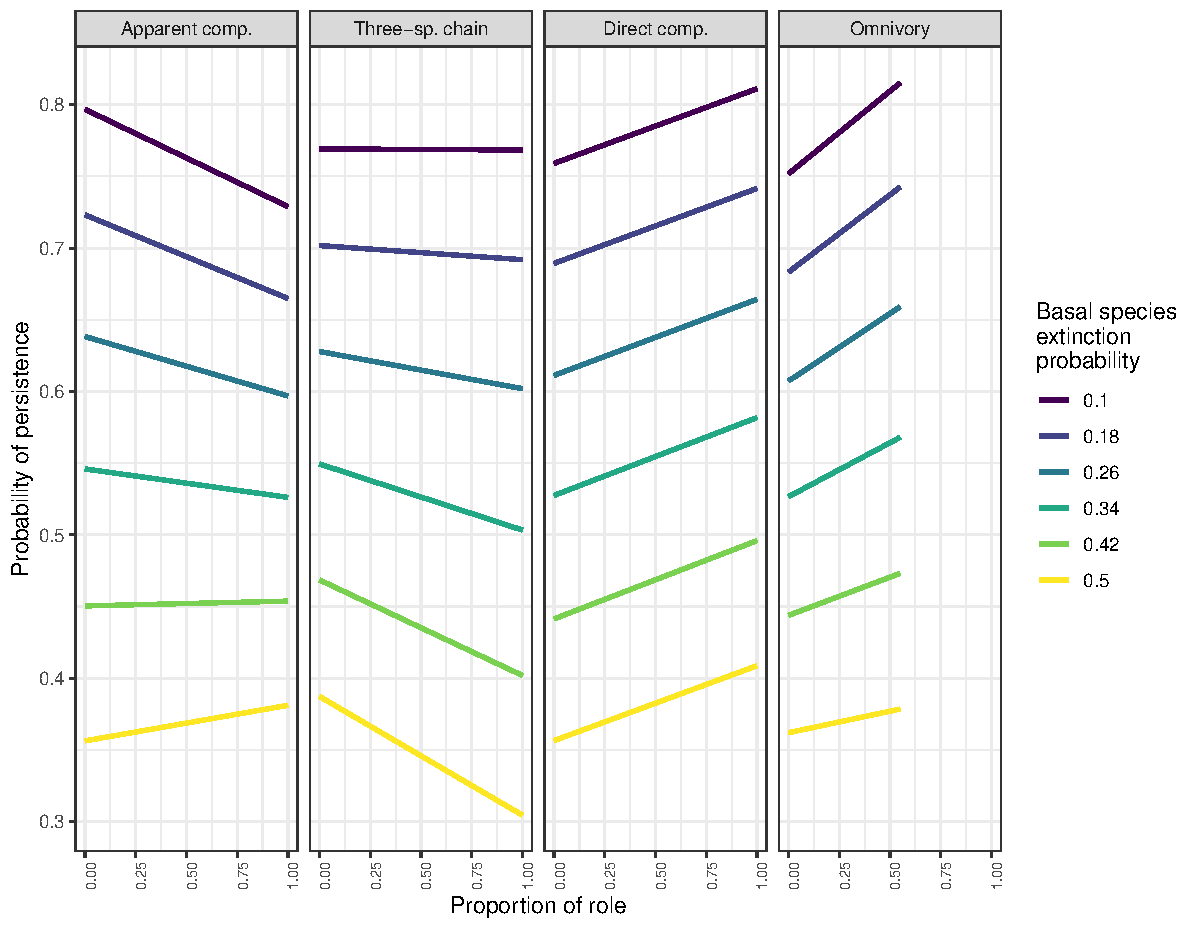
\includegraphics[width=0.85\textwidth]{figures/prop_lmer_allCS.pdf}
                \caption{The effect of proportion of the role (x-axis) made up by various motifs (columns) on persistence (y-axis). The effect of participating in each motif is based on linear mixed-effect models following Equation~\ref{propreq}, except that models for each  disturbance level are fitted separately. The different colored lines indicate the probability of extinction of basal species, from $\pi_{disturbed} = 0.1$ (top, purple; no disturbance) to $\pi_{disturbed} = 0.5$ (bottom, yellow; high disturbance). Note that omnivory made up a smaller proportion of species' roles than other motifs; lines are plotted over the observed ranges of motif participation.}
                \label{fig:prop_lmer_all}
            \end{figure}
        

    \subsection*{Motif participation and other network properties}

       Species' motif participation varied depending on the properties of the network; size, connectance, and their interaction (Fig. S4, Table S6; \emph{Appendix SG}).
       Species appeared most often in the apparent competition motif in all types of networks, but the frequency decreased with increasing network size and connectance.
       The frequency with which species participated in the omnivory motif increased sharply with increasing connectance, while the frequency of the direct competition motif increased slightly with increasing network size. 
        
       Species' motif participation also varied with their in-degree and trophic level (Fig.~\ref{fig:motifs_vs_TL_and_deg}).
       Species with higher in-degree tended to have higher frequencies of participation in the omnivory motif. Proportions of the other three motifs tended to decline with increasing degree.
       Species with higher trophic levels tended to have higher proportions of apparent competition and three-species chains. 
        
       A species persistence varies with both species in-degree and trophic level (Fig.~\ref{fig:motifs_vs_TL_and_deg}; \emph{Appendix SF}). Increased trophic level is generally associated with decreasing species persistence, although the rate of decline is slower at high disturbance (Table S5, \emph{Appendix SF}).
       In-degree shows an even stronger interaction with disturbance; having more prey species is associated with higher persistence without disturbance, but lower persistence at high levels of disturbance.
        

            \begin{figure}
                \centering
                \includegraphics[width=\textwidth]{figures/roles_vs_TL.eps}
                \caption{As with motifs, persistence varied with simpler measures of species roles in networks. Moreover, motif frequencies correlated with in-degree and trophic level. \textbf{A-B)} Persistence increased with increasing in-degree for low levels of disturbance to basal resources but decreased with increasing degree for high levels of disturbance to basal resources.
                Persistence declined with inceasing STL for all levels of disturbance to basal resources.
                \textbf{C-D)} The proportion of omnivory increased with increasing degree while all other proportions decreased. The proportions of omnivory and direct competition decreased with increasing STL while the proportions of apparent competition and three-species chains increased.}
                \label{fig:motifs_vs_TL_and_deg}
            \end{figure}        
        
    \subsection*{Consistency in effects of motif participation on species persistence}

        % In order to evaluate how consistent the relationships between a species persistence and motif participation is, and how it varies with  level of disturbance and global network structure, we fit linear regressions of species persistence against motif proportions for the species for each network separately. We then analyze the density distribution of the values of the slopes. Network size had a much smaller effect than connectance (Fig. S3; \emph{Appendix SE}); we therefore focus on connectance here. 
        
        When fitting regressions of persistence against motif participation for each network separately, networks with high connectance generally had more consistent relationships between persistence and motif participation, i.e., sharper peaks of the density distributions (Fig.~\ref{fig:density_prop_C}).
        However, this trend varied at different levels of disturbance, especially for the direct competition and omnivory motifs.
        At low and medium connectances there was little change in the distribution of slopes for direct competition across all levels of disturbance. 
        At high connectances, however, the proportion of positive slopes was both lower overall and decreased with increasing disturbance. 
        For the omnivory motif these trends were reversed. 
        Moreover, the omnivory motif has a particularly broad distribution of slopes (i.e., an inconsistent relationship to persistence) when network connectance was low. 
        Network size had a much smaller effect than connectance (Fig. S3; \emph{Appendix SE}).

        \begin{figure}[h!]
            \centering
            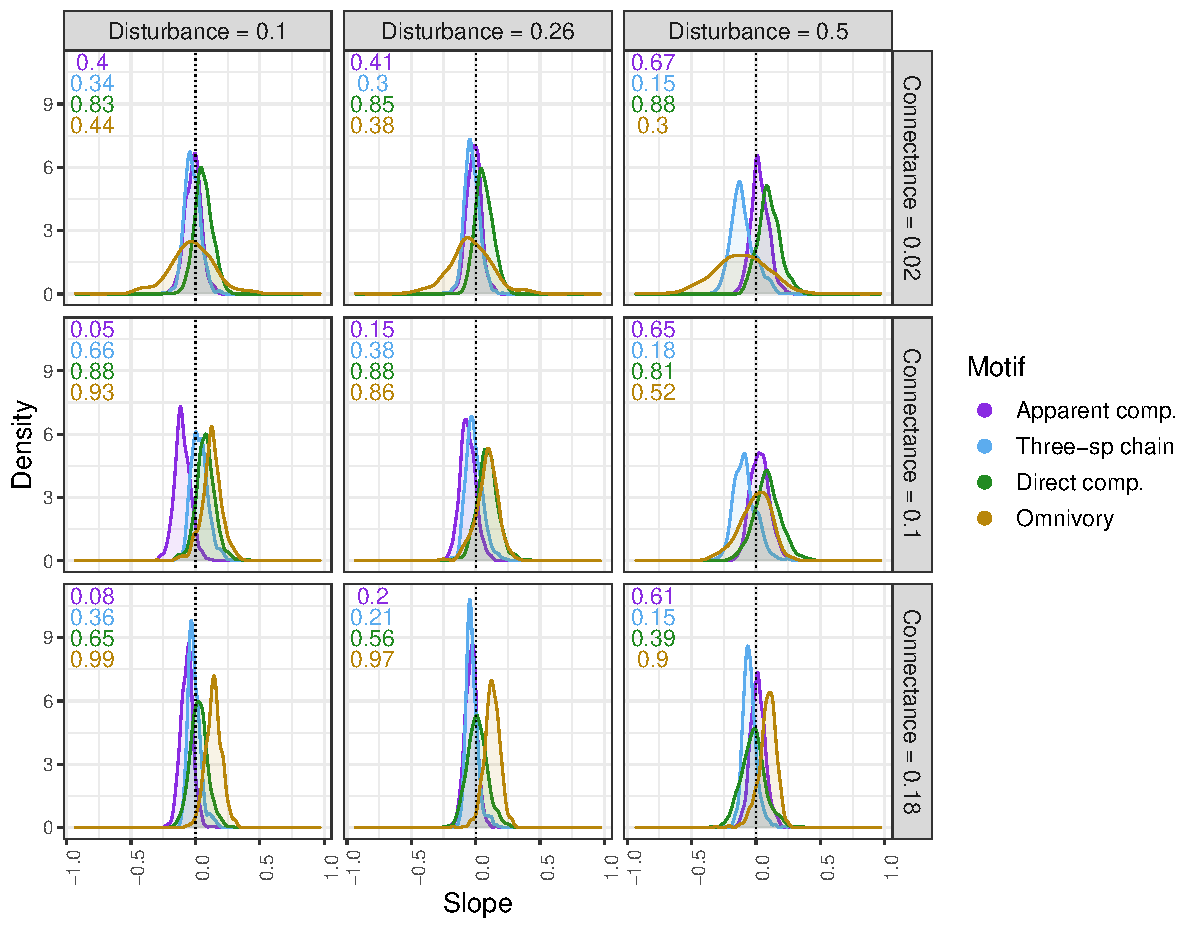
\includegraphics[width=\textwidth]{figures/prop_dens_bp_vs_C_allS.pdf}
            \caption{Here we show the density (y-axis) of slopes (x-axis) of persistence against proportion of different motifs for all simulated webs of all sizes - a visualization of how an increased proportion of each motif (different colored lines) affects persistence of consumer species. Columns show the result for various disturbances on the basal level, from $\pi_{disturbed} = 0.1$ (left) to $\pi_{disturbed} = 0.5$ (right). Rows show various levels of connectance. The dotted, vertical line indicate zero on the x-axis. A negative slope value reflects a negative relationship between increased participation in a motif and persistence, while a positive slope value reflects a positive relationship - an increased proportion of a specific motif increase persistence. The fraction of replicates with a slope greater than zero are stated in numbers in each sub-plot, the color corresponding to each motif (legend). }
            \label{fig:density_prop_C}
        \end{figure}    
    

    \subsection*{Network motif profiles and network mean persistence}
    
        The overall motif profile of a network was related to the average persistence of consumers ($F_{1,2998}$=571, $p$\textless0.001). 
        Average persistence was higher in networks with higher proportions of the chain, direct competition, and apparent competition motifs (Table S3, \emph{Appendix SC}). 
        Conversely, average persistence was lower in networks with higher proportions of the omnivory motif. 
        These trends were consistent across levels of disturbance (Fig.~\ref{fig:motif_profile_persistence}, Table S3), \emph{Appendix SC}).% Network persistence varies between networks with different dispersion of motif profiles ($F_{134,2865}$=2.19$\times10^{24}$, $p$=\textless0.001). For example, networks with more variable motif profiles have higher persistence ($\beta$=0.183, $p$\textless0.001).

        \begin{figure}
            \centering
            \includegraphics[width=.5\textwidth]{figures/persistence_motif_profiles.eps}
            \caption{The proportions of the four motifs in a network's motif profile are related to the mean persistence of species in the network. Specifically, persistence decreases as the proportion of omnivory in the network's motif profile increases while persistence increases with the proportions of the other three motifs. Interactions between motif profiles and disturbance were significant but small. Here we show the relationships of probabilities of extinction of basal resources of 0.1 (top set of lines) and 0.5 (bottom set of lines). Relationships are shown for the observed range of proportions for each motif.}      
            \label{fig:motif_profile_persistence}
        \end{figure}    


    \subsection*{Network motif profiles and global network properties}

        Although the PERMANOVA test relating overall motif profiles to network properties was not reliable (Fig. S3, \emph{Appendix SB}), 
        connectance was significantly related to the frequencies of different motifs in a network when considering motifs individually.
        Network size and the interaction between network size and connectance did not strongly affect the frequencies of most motifs (Fig.~\ref{motif_proportion_lms}).
        Considering each motif separately, the proportions of apparent competition and three-species chains in a network's motif profile tended to decrease with increasing connectance while the proportion of omnivory increased with increasing connectance (Table S2, \emph{Appendix SB}). 
    
        \begin{figure}[h!]
            \centering
            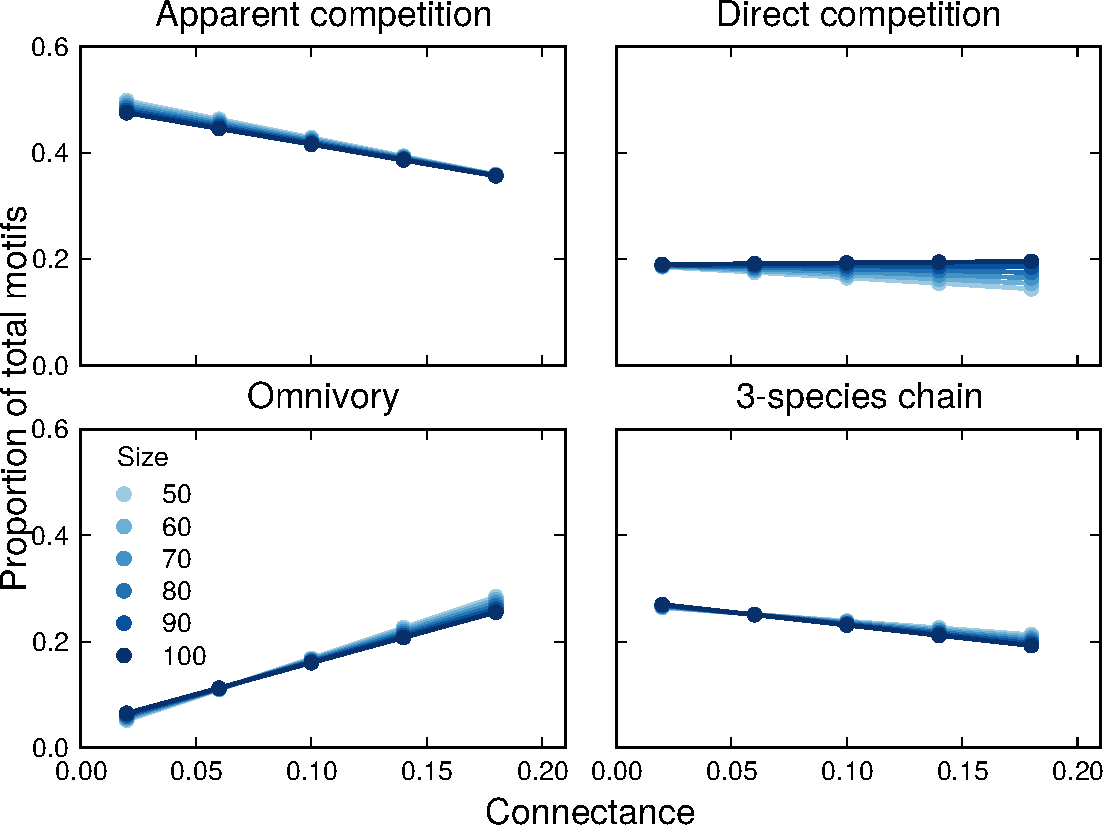
\includegraphics[width=.75\textwidth]{manuscript/figures/motif_proportion_lms.pdf}
            \caption{The proportions of the four motifs in a network's motif profile were related to the mean persistence of species in the network. Specifically, persistence decreased as the proportion of omnivory in the network's motif profile increased while persistence increased with increasing proportions of the other three motifs. Interactions between motif profiles and disturbance were significant but small. Here we show the relationships of probabilities of extinction of basal resources of 0.1 (top set of lines) and 0.5 (bottom set of lines). Relationships are shown for the observed range of proportions for each motif.}
            \label{motif_proportion_lms}
        \end{figure}


     \clearpage

\section*{Results to SI entirely?}

    \subsection*{Network mean persistence and global network properties}
    
        %Increasing the probability of extinction for basal species necessarily decreased the mean probability of persistence for consumers. 
        %This effect was clear across the ranges of network size and connectance we considered. 
        %Network size and connectance also affected network mean persistence, but to a much smaller extent than increasing disturbance (Figure S1, Table S1, \emph{Appendix SA}). 
        %Persistences generally decreased in more-connected networks, but the effect of network size varied depending on level of disturbance. 
        %At low disturbance, small and highly-connected webs showed the lowest mean persistence, whereas at high disturbance, large and highly connected webs showed the lowest mean persistence (Fig. S2, \emph{Appendix SA}).


    \subsection*{Species characteristics and persistence}
    

        % Anna notes (just for our (mine) understanding): 
        % When looking at the two figures of degree vs persistence and STL vs persistence - my conclusion is that species at lower trophic levels have the highest in-degree. Double check - yes, that’s true.
        % Lower TL are all well at low disturbances, and when disturbance increase, persistence decrease (looking at fig degree vs persistence, right end of the line).
        % Higher TL experience the same thing, although to a slightly smaller extent (looking at the left end of the lines in fig degree vs persistence and right end of lines in fig STL vs persistence). 
        % The slope of the line in fig degree vs persistence is not really relevant, since it's kind of based on the response of different TL level (which makes perfect sense in the BN framework)
        % weird thing though - at high levels of disturbance, lower TL seems more affected than higher TL in the persistence vs degree figure (since low degree belongs to higher TL, high degree to lower TL). This does not correspond with fig persistence vs STL. HOWEVER - not only high TL have a low degree, lower TL do as well, probably affecting the overall result. Only low TL have high degree - but the opposite is not true. Probably explains it
    
    \clearpage
    

    % \subsection*{Persistence and species' positioning in motifs}

    %     A species probability of persisting is significantly related to the frequency of all positions, disturbance, and the interaction between frequency of each position and disturbance (Table SX, \emph{Appendix SH}).
    %     In the omnivory motif, persistence increased with the frequency of the bottom position (two predators, no prey within the motif) across all levels of disturbance but most steeply at high levels of disturbance (Fig.~\ref{figs:persistence_position_motifs}).
    %     Persistence increased slightly with the frequency of the middle position (one prey, one predator) at low levels of disturbance but showed little relationship at higher levels of disturbance.
    %     Persistence increased with the frequency of the top position (two prey, no predators within the motif) at low disturbance but decreased at higher levels of disturbance.
        
    %     In the three-species chain, persistence decreased as the frequency of the top position increased at all levels of disturbance.
    %     Conversely, persistence increased with increasing frequency of the middle position at all levels of disturbance.
    %     Persistence decreased slightly with increasing frequency of the bottom position at low levels of disturbance but increased at high levels of disturbance.
        
    %     In the apparent competition motif, persistence decreased slightly with increasing frequencies of the bottom position (one predator, no prey within the motif) at low disturbance but increased slightly at high disturbance.
    %     Persistence increased with increasing frequency of the top position (two prey, no predator within the motif) at low disturbance but decreased at high disturbance.
        
    %     In the direct competition motif, persistence varied little with the frequency of the bottom position (two predators, no prey within the motif) at low disturbance but increased with the frequency of this position at high levels of disturbance.
    %     Persistence increased slightly with the frequency of the top position (one prey, no predators within the motif) at low levels of disturbance and decreased slightly at high levels of disturbance.
        

    % \begin{figure}[h!]
    %     \includegraphics[width=.95\textwidth]{figures/persistence_positions_Omnivory.eps}
    %     \caption{A species' probability of persistence varied with the frequency of different motif positions in its role. Here we show the relationships between persistence and the proportions of the three positions in the omnivory motif at three levels of probability of extinction for basal resources (p=0.1, 0.26, and 0.42), indicated by line colour. Line style indicates the motif  position. }
    %     \label{figs:persistence_position_motifs}
    %     \end{figure}


    %     The frequencies of motif positions in a species' role varied with network properties (\emph{Appendix SI}).Motif roles had stronger relationships with degree and STL than with network size or connectance.
        


\clearpage

%Somewhere early in discussion (needs tidying up):
%Apparent comp and direct comp have no indirect effects in BN, so we should be able to explain them with simpler properties.


\section*{Discussion}


% Focus on what additional information is revealed from analyzing motif compared to global network properties or species characteristics.
% * ADD REFS - high disturbance scenario is analogous to decreasing plant diversity

% Framing: network structure is important for predicting extinction risk

It is well known that bottom-up effects are strong in most ecosystems and that global network properties are important for how well a network can handle disturbances to those energy flows, such as loss of species \citep{Dunne2002, Eklof2006, PascualDunne2006}. 
At the same time, from a conservation perspective it is often more relevant to focus interventions on particular target species~\citep{Bottrilletal2008}. 
Nevertheless, the process of identifying target species should take the network context into account since both direct and indirect interactions can affect how species respond to a disturbance~\citep{curtsdotter2011robustness, dunne2009cascading, Eklof2006}. 


% Framing: motifs are related to network stability, species persistence (our results)
Global network properties are often too coarse grained and identification of vulnerable species in that context becomes to broad (e.g. primary producers). Motifs represent a middle-ground approach as they are the basic building blocks of networks~\citep{Milo2002}, connecting network-wide (global) and species-specific (local) properties, describing both direct and indirect effects. 
As such, the distribution of these meso-scale structures within a network is of importance to network stability ~\citep{prill2005dynamic, bascompte2005simple}.
We here show that a species' frequency of participation in different motifs is related to its probability of persistence.


% Species-level results summary
Specifically, we found that a species' probability of persistence increased with its frequency of participation in the direct competition and omnivory motifs and decreased with its frequency of participation in the three-species chain motif.
The relationship between persistence and the frequency of participation in the apparent competition motif depended strongly on the level of disturbance.
These trends can be partially explained by underlying relationships between motif participation and in-degree and/or trophic level.
For example, the frequency of participation in the direct competition motif was strongly and negatively correlated with trophic level.
Accordingly, while a high trophic level is associated with lower persistence at all levels of disturbance, the opposite is true for participation in the direct competition motif.


% Degree and TL are both important for omnivory
The relationship between participation in the omnivory motif and persistence connects motif participation with both in-degree and trophic level.
Species participation in the omnivory motif was associated with greater persistence, especially at low levels of disturbance.
This is consistent with a strong negative correlation between omnivory and trophic level (leading to the overall positive effect of omnivory) and a strong positive correlation with in-degree (leading to the reduced benefit of omnivory at high levels of disturbance). 
Motifs can, in this sense, act as a tool for synthesizing the information provided by multiple other measures of a species' place in its community, as well as interactions between the measurements.


% Degree and TL don't explain everything
Also the relationships between persistence and participation in the apparent competition and three-species chain motifs demonstrate motif participation roles' ability to syntesize different aspects of network structure.
In these cases, in-degree and trophic level are not sufficient to explain the trends we observe in the motifs.
Participation in the apparent competition motif was strongly negatively correlated with in-degree and shows a similar relationship to persistence.
However, participation in the apparent competition motif was also strongly and positively correlated with trophic level (which is negatively associated with persistence since predators by necessity have lower probability of persistence than their prey~\citep{Eklof2013}) and this correlation is not reflected in the relationship between participation in the apparent competition motif and persistence.
Similarly, participation in the three-species chain motif was significantly correlated with both in-degree and trophic level, but the relationship between the motif and persistence did not reflect the relationship between in-degree and persistence.
This suggests the influence of some other aspect of network structure on species' persistence.
As motifs capture information about direct and indirect interactions and include a larger section of the network than degree or trophic level~\citep{Cirtwill2018FoodWebs}, it is likely that effects of these indirect interactions may be included in the relationships we observe between motifs and persistence.


% Moving to network context
As well as clarifying the relationships between network structure and the effect of bottom-up disturbance on particular species, motifs were also related to the mean probability of persistence across all species in a network.
In fact, a network's motif profile had a stronger relationship to mean persistence compared to network size or connectance. 
However, connectance naturally did affect which network motifs were most common. 
For example, highly-connected networks tended to contain higher frequencies of the omnivory motif which includes more links than the other three-species motifs considered here.
Thus, global-scale properties seems to have stronger effects on network persistence by changing meso-scale properties than directly.
This in turn suggests that network motif profiles may be more useful than global network properties when predicting mean extinction risk of species in a network.
In general, we found that average network persistence was highest in networks with low frequencies of the omnivory motif and high frequencies of the apparent competition motif. These two motifs that have been shown to have consequences for the stability of ecological networks \citep{Borrelli2015a}.

% Heading into omnivory
The effect of omnivory on stability has long been a subject of debate \citep{Kratina2012}. 
Omnivory has been shown to both stabilize and destabilize communities, and the impact is highly dependent on network context \citep{bascompte2005simple, Monteiro2016}. 
For example, omnivorous interactions may not be stable in isolation but instead stabilized by interactions with other species when embedded in a larger food web \citep{Kratina2012}. 
This might be why we here find a divergent pattern between a full food web's motif profile (where a high proportion of omnivory indicates lower average network persistence) versus each single species motif profile (where a high proportion of the omnivory motif indicates a higher focal species persistence).
Thus, the ideal situation for a species could potentially be a highly omnivorous species in a low-omnivory setting. 

% High C webs and omnivory
Additionally, we show that both the presence as well as the persistence of omnivorous species are higher in high-connected networks.
The many pathways present in a high-connectance network, by which a bottom-up disturbance can propagate through the network, might explain the positive effect on persistence for species that feeds on multiple trophic levels.
%Species that participate in many omnivory motifs have feeding interactions to species at lower trophic levels in addition to the directly adjacent one. Those species will therefore be less-severely affected by these propagating disturbances enforced in high-connectance networks, in comparison to other species. 
In a sense, a species with a high proportion of omnivory will spread its risk between prey items at different trophic levels.
Although species in our model cannot swap prey dependent on bottom-level disturbances or lower resource densities, this mechanism resembles empirical studies showing that adaptive omnivory can increase the permanence of three-species chains~\citep{Fagan1997, Kvrivan2005, AbramsFung2010}.

An additional important predictor for a species persistence is its traits \citep{Brose2017, curtsdotter2011robustness, Cardillo2005, Purvis2000}. In turn, a species' set of traits also influence the likelihood of it participating in different motifs \citep{cirtwill2018feeding}. This association between motifs and traits further emphasise the role of motifs for understanding how species' roles in a network have implications for its persistence. 

There are some limitations to the approach presented here. Most important is the lack of top-down effects in the extinction risk calculations. This is because Bayesian networks operate on a strict bottom-up principle whereby prey influence their predators, but not vice versa \citep{Eklof2013}. Here our focus was to analyze the importance of disturbances to the primary producers and how effects propagate up in the food web. Earlier work indeed showed that the Bayesian network approach capture a majority of the secondary extinctions when compared to a fully-fledged dynamical model \citep{Eklof2013}, but if top-down effects are assumed important other methods should be used. Ongoing work using a dynamical model show that time to extinction for species following disturbance is tightly coupled to the species motif profile \citep{Cirtwill2021_inprep}. 

In summary, our results show that participating in different three-species motifs is related to a species' risk of extinction following a bottom-up disturbance, and that these relationships synthesize information provided by other, simpler measures of species roles.
Our results also underscore the importance of the level of disturbance when identifying which species are most at risk of extinction.
There were strong interactions between the level of disturbance and the relationships between persistence and measures of species roles (motifs and in-degree).
These simulated results echo empirical studies which report `tipping points' where previously beneficial traits can become risky~\citep{}.
These disturbance effects mean that efforts to define a set of target species for conservation interactions must take the current (and future) level of disturbance the community experiences into account.


\clearpage    

\section*{Glossary}

\begin{table}[h!]
\label{glossary}
\caption{Glossary of terms relating to motifs and Bayesian networks}

\begin{tabular}{l|l}
    Term & Definition \\
    \hline
    Motif &  \\
    Network profile & \\
    Motif participation & \\
    Motif role & \\
    Bayesian network & A directed acyclic graph, used to predict species' likelihood of persistence. \\
    Network persistence & The mean likelihood of consumers in a network not going extinct.\\
    Species persistence & The individual likelihood of a species not going extinct.\\
    In-degree & Number of prey species to a consumer species.\\
    Trophic level (STL) & The shortest food chain between the focal species and any basal species.\\
    Disturbance ($\pi_{disturbed}$) & Probability of extinction of a basal resource when extra disturbance is added. \\
    Baseline extinction &  When no disturbance is applied, $\pi_{base}$=0.1.\\
\end{tabular}
\end{table}

% Notes on what expressions and words to use
% "probability of extinction" or "level of disturbance" for the different disturbace scenarios?


\bibliographystyle{ecollett} 
\bibliography{anna_bib_new} % Abbreviate journal titles.

\end{spacing}

\end{document}

